% Bab 3  Metodologi/Perancangan
\chapter{METODOLOGI/PERANCANGAN}

\section{Perancangan dan Pengujian}
Bagian ini menjelaskan perancangan sistem yang digunakan, cara mengimplementasikan rancangan, dan cara pengujian sistem (indikator kinerja dan cara mengukurnya). Penjelasan ini bisa terdiri dari beberapa subbab yang saling terkait.

Contoh kalimat bersitasi: Prosedur pengujian mengacu pada penelitian sebelumnya (AlQahtani \& Alhassany, 2013).

Alat dan bahan yang akan digunakan dapat disajikan dalam tabel, seperti Tabel 3.1 (data contoh).

\begin{singlespace}
\begin{longtable}{|c|p{0.26\linewidth}|p{0.30\linewidth}|c|}
\caption{Contoh daftar alat dan bahan penelitian}\\
\hline
\textbf{No.} & \textbf{Nama} & \textbf{Spesifikasi} & \textbf{Jumlah} \\
\hline
1 & Papan ESP32 & Dua inti 240 MHz, Wi-Fi 2,4 GHz & 1 \\
\hline
2 & Sensor DHT22 & Suhu $-40$ sampai 80 $^\circ$C, galat $\pm$0,5 $^\circ$C & 3 \\
\hline
3 & Modul relay & 5 V, satu kanal & 1 \\
\hline
4 & Layar LCD 16$\times$2 & Antarmuka I2C & 1 \\
\hline
\end{longtable}
\end{singlespace}

Tahapan penelitian dapat digambarkan dengan diagram alir, seperti Gambar 3.1, dan rancangan perangkat keras dengan skema rangkaian, seperti Gambar 3.2 (isi kedua gambar adalah contoh).

\begin{figure}[H]
\centering
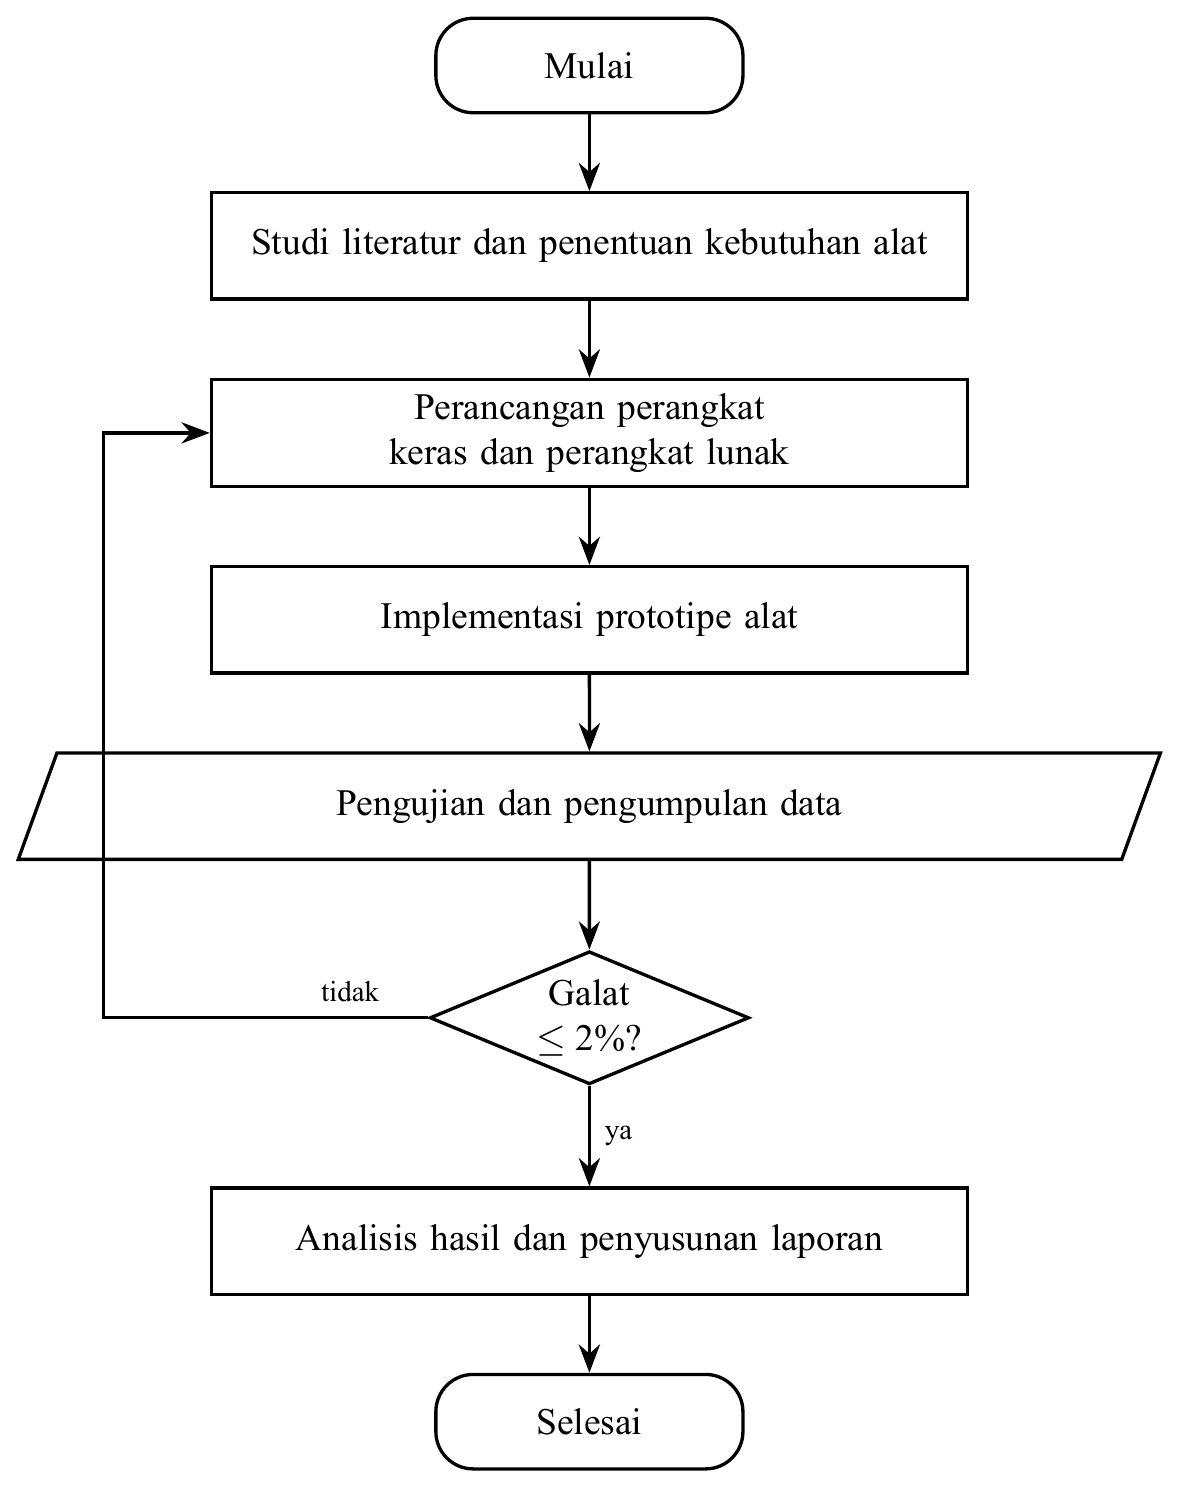
\includegraphics[width=0.5\textwidth]{../00-gambar/contoh-alur.png}
\caption{Contoh diagram alir tahapan penelitian}
\end{figure}

\begin{figure}[H]
\centering
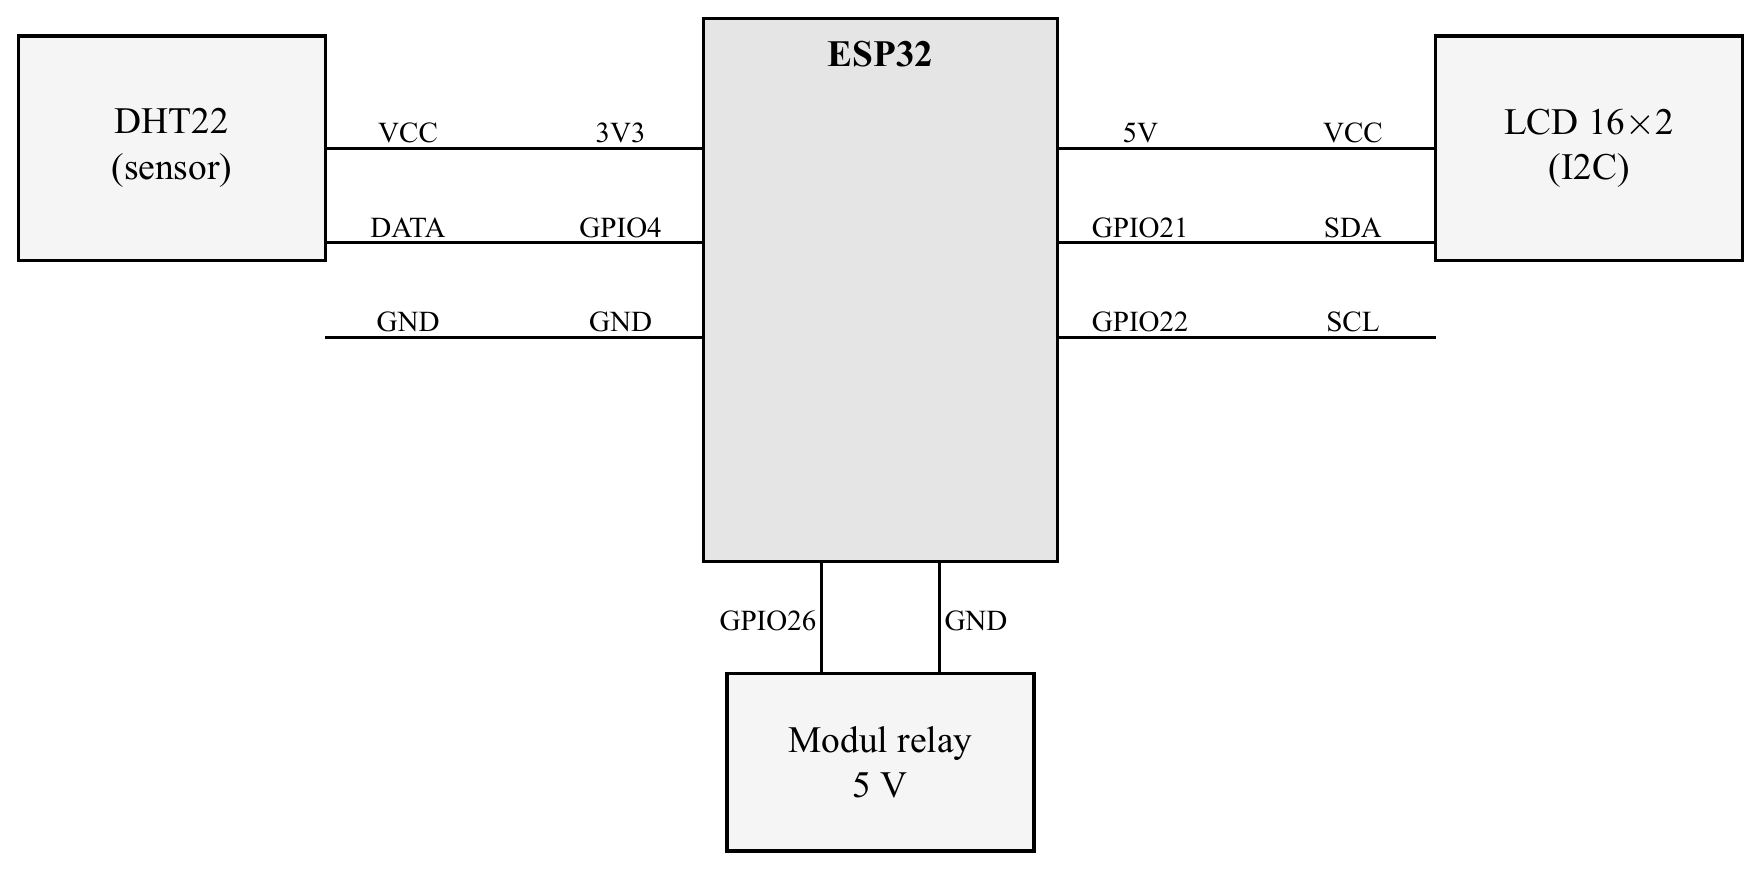
\includegraphics[width=0.95\textwidth]{../00-gambar/contoh-rangkaian.png}
\caption{Contoh skema rangkaian perangkat keras}
\end{figure}

\needspace{10cm}
\section{Jadwal Pelaksanaan}
Buatlah jadwal aktivitas berdasarkan tahapan penyelesaian skripsi Anda dalam waktu 6 bulan.

\begin{table}[H]
\caption{Jadwal pelaksanaan penelitian}
\centering
\begin{singlespace}
\renewcommand{\arraystretch}{1.8}
\setlength{\tabcolsep}{9pt}
\begin{tabular}{|c|p{4.8cm}|*{6}{c|}}
\hline
\multirow{2}{*}{\textbf{No}} & \multirow{2}{*}{\textbf{Deskripsi Kegiatan}} & \multicolumn{6}{c|}{\textbf{202x}} \\
\cline{3-8}
 & & 1 & 2 & 3 & 4 & 5 & 6 \\
\hline
1 & Kegiatan 1 & \isi & & & & & \\
\hline
2 & Kegiatan 2 & \isi & \isi & & & & \\
\hline
3 & Kegiatan 3 & & \isi & \isi & & & \\
\hline
4 & Kegiatan 4 & & & \isi & \isi & & \\
\hline
5 & Kegiatan 5 & & & & \isi & & \\
\hline
6 & Kegiatan 6 & & & & & \isi & \isi \\
\hline
\end{tabular}
\end{singlespace}
\end{table}
